\documentclass{article}

\usepackage{tikz} 
\usetikzlibrary{automata, positioning, arrows} 

\usepackage{amsthm}
\usepackage{amsfonts}
\usepackage{amsmath}
\usepackage{amssymb}
\usepackage{fullpage}
\usepackage{color}
\usepackage{parskip}
\usepackage{hyperref}
  \hypersetup{
    colorlinks = true,
    urlcolor = blue,       % color of external links using \href
    linkcolor= blue,       % color of internal links 
    citecolor= blue,       % color of links to bibliography
    filecolor= blue,        % color of file links
    }
    
\usepackage{listings}
\usepackage[utf8]{inputenc}                                                    
\usepackage[T1]{fontenc}   
\usepackage[margin=1in]{geometry}
\usepackage{tikz}
\usepackage{caption}
\captionsetup[figure]{labelformat=empty}
\usetikzlibrary{arrows.meta,positioning}
\tikzset{
  >=Stealth,
  obj/.style = {circle, draw, minimum size=8mm, inner sep=0pt, font=\small},
}
\newcommand{\rowlabel}[3]{\textbf{Confluent #1,\ Terminating #2,\ Unique NFs #3}}

\definecolor{dkgreen}{rgb}{0,0.6,0}
\definecolor{gray}{rgb}{0.5,0.5,0.5}
\definecolor{mauve}{rgb}{0.58,0,0.82}

\lstset{frame=tb,
  language=haskell,
  aboveskip=3mm,
  belowskip=3mm,
  showstringspaces=false,
  columns=flexible,
  basicstyle={\small\ttfamily},
  numbers=none,
  numberstyle=\tiny\color{gray},
  keywordstyle=\color{blue},
  commentstyle=\color{dkgreen},
  stringstyle=\color{mauve},
  breaklines=true,
  breakatwhitespace=true,
  tabsize=3
}

\newtheoremstyle{theorem}
  {\topsep}   % ABOVESPACE
  {\topsep}   % BELOWSPACE
  {\itshape\/}  % BODYFONT
  {0pt}       % INDENT (empty value is the same as 0pt)
  {\bfseries} % HEADFONT
  {.}         % HEADPUNCT
  {5pt plus 1pt minus 1pt} % HEADSPACE
  {}          % CUSTOM-HEAD-SPEC
\theoremstyle{theorem} 
   \newtheorem{theorem}{Theorem}[section]
   \newtheorem{corollary}[theorem]{Corollary}
   \newtheorem{lemma}[theorem]{Lemma}
   \newtheorem{proposition}[theorem]{Proposition}
\theoremstyle{definition}
   \newtheorem{definition}[theorem]{Definition}
   \newtheorem{example}[theorem]{Example}
\theoremstyle{remark}    
  \newtheorem{remark}[theorem]{Remark}

\title{CPSC-354 Report}
\author{Mitchell Toney  \\ Chapman University}

\date{\today} 

\begin{document}

\maketitle

\begin{abstract}
\end{abstract}

\setcounter{tocdepth}{3}
\tableofcontents

\section{Introduction}\label{intro}

\section{Week by Week}\label{homework}

\subsection{Week 1: HW1}
The $MU$ puzzle is a puzzle created by Douglas Hofstadter. It consists of four rules that can be applied to a string $MI$.
\[
\begin{array}{l}
1.\ xI \rightarrow xIU \\
2.\ Mx \rightarrow Mxx \\
3.\ xIIIy \rightarrow xUy \\
4.\ xUUy \rightarrow xy 
\end{array}
\]
When first approaching this puzzle, the first strategy that came to mind was to take advantage of rule number 2 to keep duplicating the I's until there is a multiple of three, then using rules 3 and 4 to get rid of the I's and leave a remaining U.

The issue with this is that $2^{n}\bmod 3$ will never equal 0, it infinitely cycles between equaling 1 and 2, and without being able to get rid of all the I's, which would require them being a multiple of 3, you will never be able to get MU.

Thus, the puzzle is not solvable.

\subsection{Week 2: HW2}


\begin{center}

% Drawing 1
\begin{minipage}{0.28\textwidth}\centering
\begin{tikzpicture}
  \draw[dashed, rounded corners] (-0.9,-0.9) rectangle (1.1,0.9);
\end{tikzpicture}
\captionof{figure}{1.\; \(A=\varnothing,\; R=\varnothing\)}
\end{minipage}\hfill
% Drawing 2
\begin{minipage}{0.28\textwidth}\centering
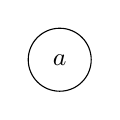
\begin{tikzpicture}
  \node[obj] (a) at (0,0) {$a$};
\end{tikzpicture}
\captionof{figure}{2.\; \(A=\{a\},\; R=\varnothing\)}
\end{minipage}\hfill
% Drawing 3
\begin{minipage}{0.28\textwidth}\centering
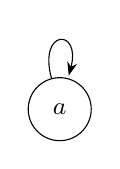
\begin{tikzpicture}
  \node[obj] (a) at (0,0) {$a$};
  \path (a) edge[loop above] (a); % (a,a)
\end{tikzpicture}
\captionof{figure}{3.\; \(A=\{a\},\; R=\{(a,a)\}\)}
\end{minipage}

\vspace{1em}

% Drawing 4
\begin{minipage}{0.28\textwidth}\centering
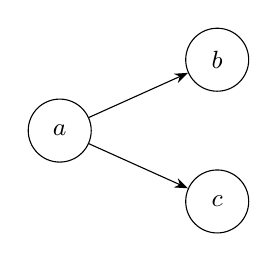
\begin{tikzpicture}
  \node[obj] (a) at (0,0) {$a$};
  \node[obj] (b) at (2,0.9) {$b$};
  \node[obj] (c) at (2,-0.9) {$c$};
  \draw[->] (a) -- (b);  % (a,b)
  \draw[->] (a) -- (c);  % (a,c)
\end{tikzpicture}
\captionof{figure}{4.\; \(A=\{a,b,c\},\; R=\{(a,b),(a,c)\}\)}
\end{minipage}\hfill
% Drawing 5
\begin{minipage}{0.28\textwidth}\centering
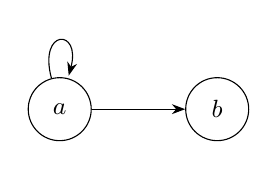
\begin{tikzpicture}
  \node[obj] (a) at (0,0) {$a$};
  \node[obj] (b) at (2,0) {$b$};
  \path (a) edge[loop above] (a); % (a,a)
  \draw[->] (a) -- (b);          % (a,b)
\end{tikzpicture}
\captionof{figure}{5.\; \(A=\{a,b\},\; R=\{(a,a),(a,b)\}\)}
\end{minipage}\hfill
% Drawing 6
\begin{minipage}{0.28\textwidth}\centering
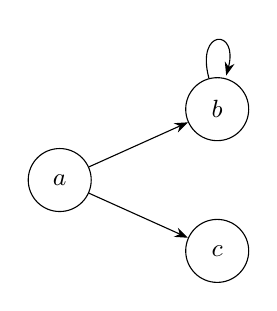
\begin{tikzpicture}
  \node[obj] (a) at (0,0) {$a$};
  \node[obj] (b) at (2,0.9) {$b$};
  \node[obj] (c) at (2,-0.9) {$c$};
  \draw[->] (a) -- (b);       % (a,b)
  \draw[->] (a) -- (c);       % (a,c)
  \path (b) edge[loop above] (b); % (b,b)
\end{tikzpicture}
\captionof{figure}{6.\; \(A=\{a,b,c\},\; R=\{(a,b),(b,b),(a,c)\}\)}
\end{minipage}

\vspace{1em}

% Drawing 7
\begin{minipage}{0.28\textwidth}\centering
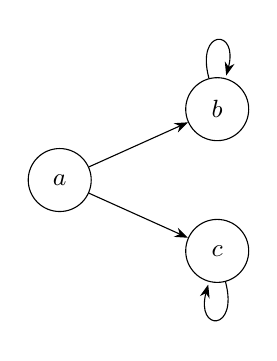
\begin{tikzpicture}
  \node[obj] (a) at (0,0) {$a$};
  \node[obj] (b) at (2,0.9) {$b$};
  \node[obj] (c) at (2,-0.9) {$c$};
  \draw[->] (a) -- (b);            % (a,b)
  \draw[->] (a) -- (c);            % (a,c)
  \path (b) edge[loop above] (b);  % (b,b)
  \path (c) edge[loop below] (c);  % (c,c)
\end{tikzpicture}
\captionof{figure}{7.\; \(A=\{a,b,c\},\; R=\{(a,b),(b,b),(a,c),(c,c)\}\)}
\end{minipage}

\end{center}

\[
\begin{array}{c|c|c|c}
\text{\#} & \text{Terminating} & \text{Confluent} & \text{Unique NFs}\\\hline
1 & \text{Yes} & \text{Yes} & \text{Yes}\\
2 & \text{Yes} & \text{Yes} & \text{Yes}\\
3 & \text{No}  & \text{Yes} & \text{No}\\
4 & \text{Yes} & \text{No}  & \text{No}\\
5 & \text{No}  & \text{Yes} & \text{Yes}\\
6 & \text{No}  & \text{No}  & \text{No}\\
7 & \text{No}  & \text{No}  & \text{No}
\end{array}
\]

\noindent\rule{\textwidth}{0.4pt}

\begin{center}

% Row 1
\begin{minipage}{0.45\textwidth}\centering
\rowlabel{True}{True}{True}\par\vspace{0.35em}
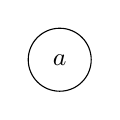
\begin{tikzpicture}
  \node[obj] (a) at (0,0) {$a$};
\end{tikzpicture}

$A=\{a\},\ R=\varnothing$
\end{minipage}\hfill
% Row 2
\begin{minipage}{0.45\textwidth}\centering
\rowlabel{True}{True}{False}\par\vspace{0.35em}
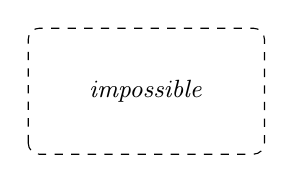
\begin{tikzpicture}
  \draw[dashed, rounded corners] (-1.5,-0.8) rectangle (1.5,0.8);
  \node at (0,0) {\small \emph{impossible}};
\end{tikzpicture}

(no ARS exists)
\end{minipage}

\vspace{1.2em}

% Row 3
\begin{minipage}{0.45\textwidth}\centering
\rowlabel{True}{False}{True}\par\vspace{0.35em}
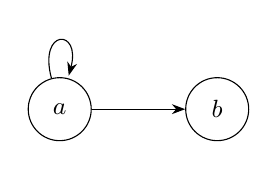
\begin{tikzpicture}
  \node[obj] (a) at (0,0) {$a$};
  \node[obj] (b) at (2,0) {$b$};
  \path (a) edge[loop above] (a);
  \draw[->] (a) -- (b);
\end{tikzpicture}

$A=\{a,b\},\ R=\{(a,a),(a,b)\}$
\end{minipage}\hfill
% Row 4
\begin{minipage}{0.45\textwidth}\centering
\rowlabel{True}{False}{False}\par\vspace{0.35em}
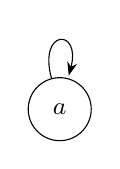
\begin{tikzpicture}
  \node[obj] (a) at (0,0) {$a$};
  \path (a) edge[loop above] (a);
\end{tikzpicture}

$A=\{a\},\ R=\{(a,a)\}$
\end{minipage}

\vspace{1.2em}

% Row 5
\begin{minipage}{0.45\textwidth}\centering
\rowlabel{False}{True}{True}\par\vspace{0.35em}
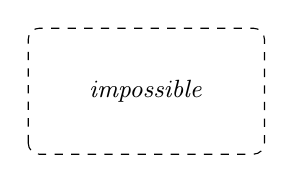
\begin{tikzpicture}
  \draw[dashed, rounded corners] (-1.5,-0.8) rectangle (1.5,0.8);
  \node at (0,0) {\small \emph{impossible}};
\end{tikzpicture}

(no ARS exists)
\end{minipage}\hfill
% Row 6
\begin{minipage}{0.45\textwidth}\centering
\rowlabel{False}{True}{False}\par\vspace{0.35em}
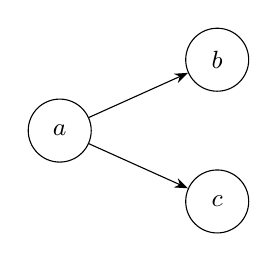
\begin{tikzpicture}
  \node[obj] (a) at (0,0) {$a$};
  \node[obj] (b) at (2,0.9) {$b$};
  \node[obj] (c) at (2,-0.9) {$c$};
  \draw[->] (a) -- (b);
  \draw[->] (a) -- (c);
\end{tikzpicture}

$A=\{a,b,c\},\ R=\{(a,b),(a,c)\}$
\end{minipage}

\vspace{1.2em}

% Row 7
\begin{minipage}{0.45\textwidth}\centering
\rowlabel{False}{False}{True}\par\vspace{0.35em}
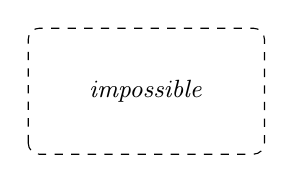
\begin{tikzpicture}
  \draw[dashed, rounded corners] (-1.5,-0.8) rectangle (1.5,0.8);
  \node at (0,0) {\small \emph{impossible}};
\end{tikzpicture}

(no ARS exists)
\end{minipage}\hfill
% Row 8
\begin{minipage}{0.45\textwidth}\centering
\rowlabel{False}{False}{False}\par\vspace{0.35em}
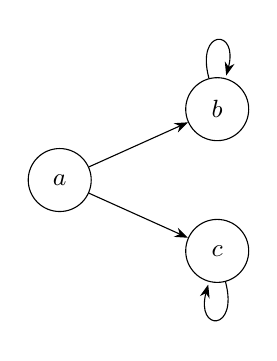
\begin{tikzpicture}
  \node[obj] (a) at (0,0) {$a$};
  \node[obj] (b) at (2,0.9) {$b$};
  \node[obj] (c) at (2,-0.9) {$c$};
  \draw[->] (a) -- (b);
  \draw[->] (a) -- (c);
  \path (b) edge[loop above] (b);
  \path (c) edge[loop below] (c);
\end{tikzpicture}

$A=\{a,b,c\},\ R=\{(a,b),(a,c),(b,b),(c,c)\}$
\end{minipage}

\end{center}

\subsection{Week 3: HW3}

\subsubsection{Exercise 5}

Consider rewrite rules:
\begin{align*}
ab &\rightarrow ba \\
ba &\rightarrow ab \\
aa &\rightarrow\\
b &\rightarrow
\end{align*}

 
\subsubsection*{Example Reductions}


\textbf{Reducing \texttt{abba}:}
\begin{align*}
abba &\rightarrow baba \quad \text{(using } ab \rightarrow ba\text{)} \\
baba &\rightarrow bbaa \quad \text{(using } ba \rightarrow ab\text{)} \\
bbaa &\rightarrow baa \quad \text{(using } b \rightarrow \varepsilon\text{)} \\
baa &\rightarrow aba \quad \text{(using } ba \rightarrow ab\text{)} \\
aba &\rightarrow baa \quad \text{(using } ab \rightarrow ba\text{)}
\end{align*}
There is an infinite loop between \texttt{aba} and \texttt{baa}.

\textbf{Reducing \texttt{bababa}:}
\begin{align*}
bababa &\rightarrow ababab \quad \text{(using } ba \rightarrow ab\text{)} \\
ababab &\rightarrow baabab \quad \text{(using } ab \rightarrow ba\text{)} \\
baabab &\rightarrow ababab \quad \text{(using } ba \rightarrow ab\text{)}
\end{align*}
This is an infinite loop between \texttt{ababab} and \texttt{baabab}.

\paragraph{Why the ARS is not terminating}

The ARS is not terminating because the rules $ab \rightarrow ba$ and $ba \rightarrow ab$ create infinite cycles. These rules allow us to swap adjacent $a$ and $b$ characters indefinitely, leading to non-terminating reduction sequences.

\paragraph{Non-equivalent strings}

Two strings that are not equivalent: \texttt{a} and \texttt{aa}. 

The string \texttt{a} cannot be reduced further, while \texttt{aa} reduces to nothing using the rule $aa \rightarrow $. Since $nothing \neq a$, these strings are in different equivalence classes.

\paragraph{Equivalence classes}

The equivalence relation $\leftrightarrow^*$ has infinitely many equivalence classes. Each equivalence class can be characterized by the number of $a$'s modulo 2 and the number of $b$'s modulo 1.

The equivalence classes are:
\begin{itemize}
\item $[\varepsilon]$: strings with even number of $a$'s and no $b$'s
\item $[a]$: strings with odd number of $a$'s and no $b$'s  
\item $[b]$: strings with any number of $a$'s and at least one $b$
\end{itemize}

The normal forms are: $\varepsilon$, $a$, and $b$.

\paragraph{Modifying the ARS to be terminating}

To make the ARS terminating without changing equivalence classes, we can remove the symmetric rules and keep only one direction:

\begin{align*}
ba &\rightarrow ab \\
aa &\rightarrow \varepsilon \\
b &\rightarrow \varepsilon
\end{align*}

This eliminates the infinite cycles while preserving the same equivalence relation.

\subsubsection{Semantic question}


\textbf{Parity of $a$'s:} "Does this string contain an odd number of $a$'s?" \\
Answer: Yes if the normal form is $a$, No if the normal form is $\varepsilon$.

\subsubsection*{Exercise 5b}

Consider rewrite rules:
\begin{align*}
ab &\rightarrow ba \\
ba &\rightarrow ab \\
aa &\rightarrow a \\
b &\rightarrow
\end{align*}

\textbf{Reducing \texttt{abba}:}
\begin{align*}
abba &\rightarrow baba \\
baba &\rightarrow abba
\end{align*}

\textbf{Reducing \texttt{bababa}:}
\begin{align*}
bababa &\rightarrow ababab \\
ababab &\rightarrow bababa
\end{align*}

\textbf{Why not terminating.} The symmetric swaps $ab \leftrightarrow ba$ allow infinite rewriting.

\textbf{Non-equivalent strings.} $a$ and $\varepsilon$ are not equivalent.

\textbf{Equivalence classes.} Exactly two: $[\varepsilon]$ (no $a$'s; all $b$'s delete) and $[a]$ (at least one $a$; since $aa \sim a$).
Normal forms (under a terminating orientation): $\varepsilon$ and $a$.

\textbf{Terminating variant.}
\begin{align*}
ba &\rightarrow ab \\
aa &\rightarrow a \\
b &\rightarrow
\end{align*}


This gives a complete semantics to the ARS: it computes the invariant for any input string.

\subsection{Week 4: HW4}

\subsubsection{HW4.1: Termination Proof for GCD}

Consider the following algorithm:

\begin{verbatim}
while b != 0:
    temp = b
    b = a mod b
    a = temp
return a
\end{verbatim}

\textbf{Assume:} Work over integers with Euclidean division: inputs $a\in\mathbb Z$, $b\in\mathbb N$; if $b\neq 0$ then $0\le a\bmod b<b$.

\textbf{Model:} States $A=\mathbb Z\times\mathbb N$. One step $(a,b)\to(a',b')$ is one loop iteration.

\textbf{Measure:} $\phi:A\to\mathbb N,\;\phi(a,b)=b$.

\textbf{Show:} $(a,b)\to(a',b') \Rightarrow \phi(a',b')<\phi(a,b)$.

If $b\neq 0$, the update sets $b'=a\bmod b$ with $0\le b'<b$; hence $\phi(a',b')=b'<b=\phi(a,b)$.

$\phi$ strictly decreases in $\mathbb N$, so there is no infinite $\to$-chain; eventually $b=0$ and the loop stops. Thus the algorithm terminates under the stated conditions.

\subsubsection{HW4.2: Termination Proof for Merge Sort}

Consider the following fragment of an implementation of merge sort:

\begin{verbatim}
function merge_sort(arr, left, right):
    if left >= right:
        return
    mid = (left + right) / 2
    merge_sort(arr, left, mid)
    merge_sort(arr, mid+1, right)
    merge(arr, left, mid, right)
\end{verbatim}

Prove that 

$\phi(\texttt{left}, \texttt{right}) = \texttt{right} - \texttt{left} + 1$ 

is a measure function for merge\_sort.

\textbf{Show:} For

\begin{verbatim}
merge_sort(arr, left, right):
  if left >= right: return
    mid = floor((left + right)/2)
  merge_sort(arr, left, mid)
  merge_sort(arr, mid+1, right)
  merge(arr, left, mid, right)
\end{verbatim}


the function $\phi(\text{left},\text{right})=\text{right}-\text{left}+1$ is a strictly decreasing measure, hence \texttt{merge\_sort} terminates.

\textbf{Assume:} \texttt{left,right}$\in\mathbb{Z}$ with $0\le \text{left}\le \text{right}<|arr|$. Division for \texttt{mid} is integer. If \texttt{left < right}, then $\text{left}\le \text{mid}<\text{right}$. \texttt{merge} makes no recursive calls.

\textbf{Model:} States are intervals $A=\{(l,r)\in\mathbb Z^2\mid l\le r\}$. A "step" is a recursive edge from $(l,r)$ (with $l<r$) to each child $(l,\text{mid})$ and $(\text{mid}+1,r)$.

\textbf{Measure:} $\phi:A\to\mathbb N,\quad \phi(l,r)=r-l+1$.

Let $l<r$ and $\text{mid}=\lfloor(l+r)/2\rfloor$ so $l\le \text{mid}<r$.

First child: $\phi(l,\text{mid})=\text{mid}-l+1\le (r-1)-l+1=r-l=\phi(l,r)-1<\phi(l,r)$.

Second child: $\phi(\text{mid}+1,r)=r-\text{mid}\le r-l=\phi(l,r)-1<\phi(l,r)$.

Every recursive edge strictly decreases $\phi$ in $\mathbb N$, which is well-founded. Thus no infinite recursion is possible; the calls bottom out at states with $\phi\in\{0,1\}$ (i.e., \texttt{left $\geq$ right}), where the function returns. Therefore $\phi(\text{left},\text{right})=\text{right}-\text{left}+1$ is a valid measure and \texttt{merge\_sort} terminates under the stated conditions.

\subsection{Week 5: HW5}

\subsubsection{Lambda Calculus Workout Evaluation (Corrected)}

Evaluate: $(\lambda f.\lambda x.\,f(f\,x))(\lambda g.\lambda y.\,g(g(g\,y)))$

Use $\alpha$-renaming to avoid capture.

\[
\begin{aligned}
(\lambda f.\lambda x.\,f(f\,x))(\lambda g.\lambda y.\,g(g(g\,y)))
&\to \lambda x.\,(\lambda g.\lambda y.\,g(g(g\,y)))\big((\lambda g.\lambda y.\,g(g(g\,y)))\,x\big)\\
(\lambda g.\lambda y.\,g(g(g\,y)))\,x
&\to \lambda y.\,x(x(x\,y)) \quad (\text{$\alpha$-rename inner } y)\\
\Rightarrow\ \lambda x.\,(\lambda g.\lambda y.\,g(g(g\,y)))\,(\lambda y.\,x(x(x\,y)))
&\to \lambda x.\lambda y.\,x^9 y.
\end{aligned}
\]

Hence the normal form is $\lambda f.\lambda x.\,f^{9}x$ (Church numeral $9$).

\section{Essay}

\section{Evidence of Participation}

\section{Conclusion}\label{conclusion}

\begin{thebibliography}{99}
\bibitem[BLA]{bla} Author, \href{https://en.wikipedia.org/wiki/LaTeX}{Title}, Publisher, Year.
\end{thebibliography}

\end{document}
